\documentclass[../main.tex]{subfiles}

\begin{document}

\subsubsection{Raspored trenera}
Trener svoje treninge vidi kao tabelu za svaki dan u nedelji koji izabere \ref{fig:trener_raspored}. Trener Inicijalno vidi svoj raspored treninga za ponedeljak, ali može videti svoj raspored za bilo koji drugi dan, birajući odgovarajuće polje za taj dan u nedelji iznad tabele.

\begin{figure}[!ht]
\begin{center}
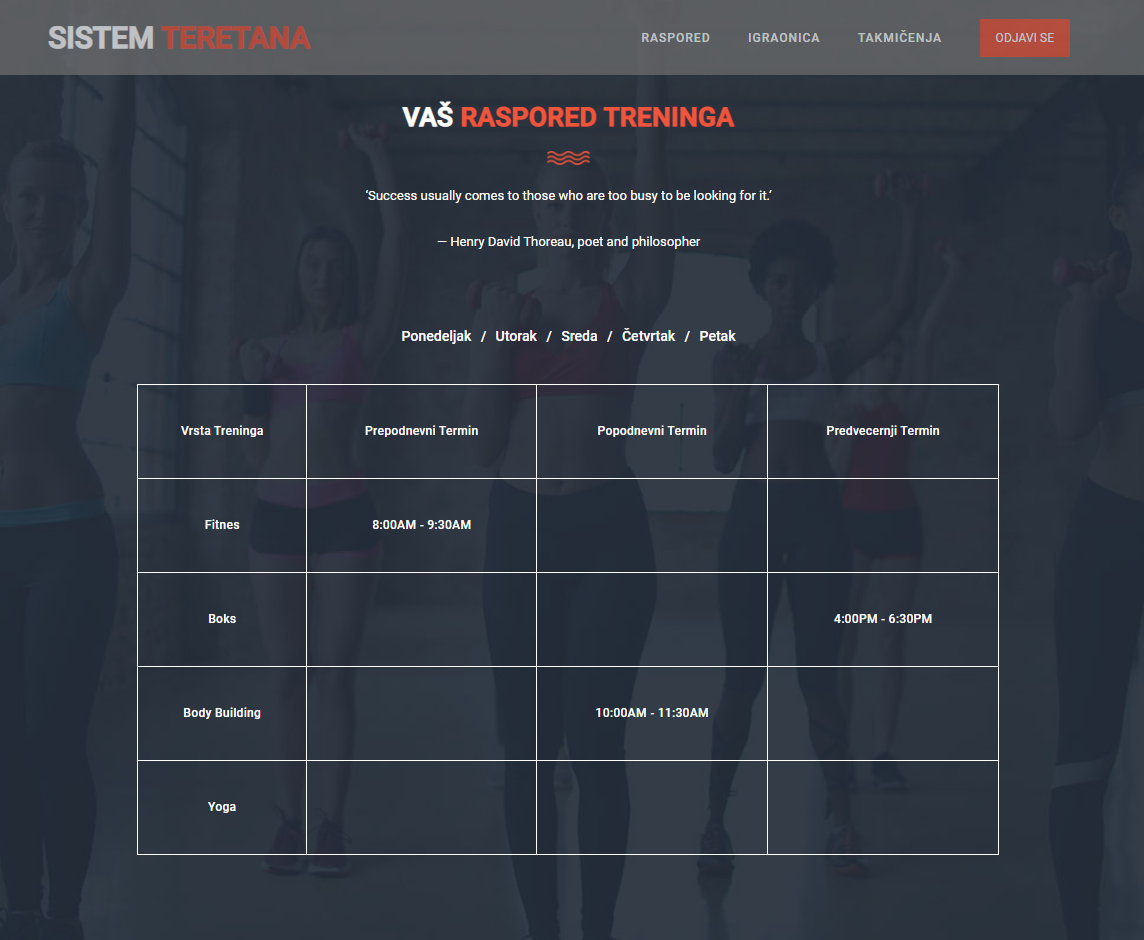
\includegraphics[scale=0.35]{sections/korisnicki_interfejs/screenshots/trener_raspored_init.PNG}
\end{center}
\caption{Raspored trenera}
\label{fig:trener_raspored}
\end{figure}


Zakazani trening je popunjeno polje u tabeli na preseku kolona, koje predtavljaju doba dana u kom je trening zakazan, i vrsti, koje predstavljaju vrste treninga koje drži. Trener može da klikne na prazno polje u tabeli ako želi da doda novi trening (\ref{fig:trener_toolbar} desno, \ref{fig:trener_forme} poslednja ) ili da klikne na već rezervisan trening (\ref{fig:trener_toolbar} levo) u oba slučaja se iznad tabele prikazuje traka sa odgovarajućim alatkama. 

\begin{figure}[!ht]
\begin{center}
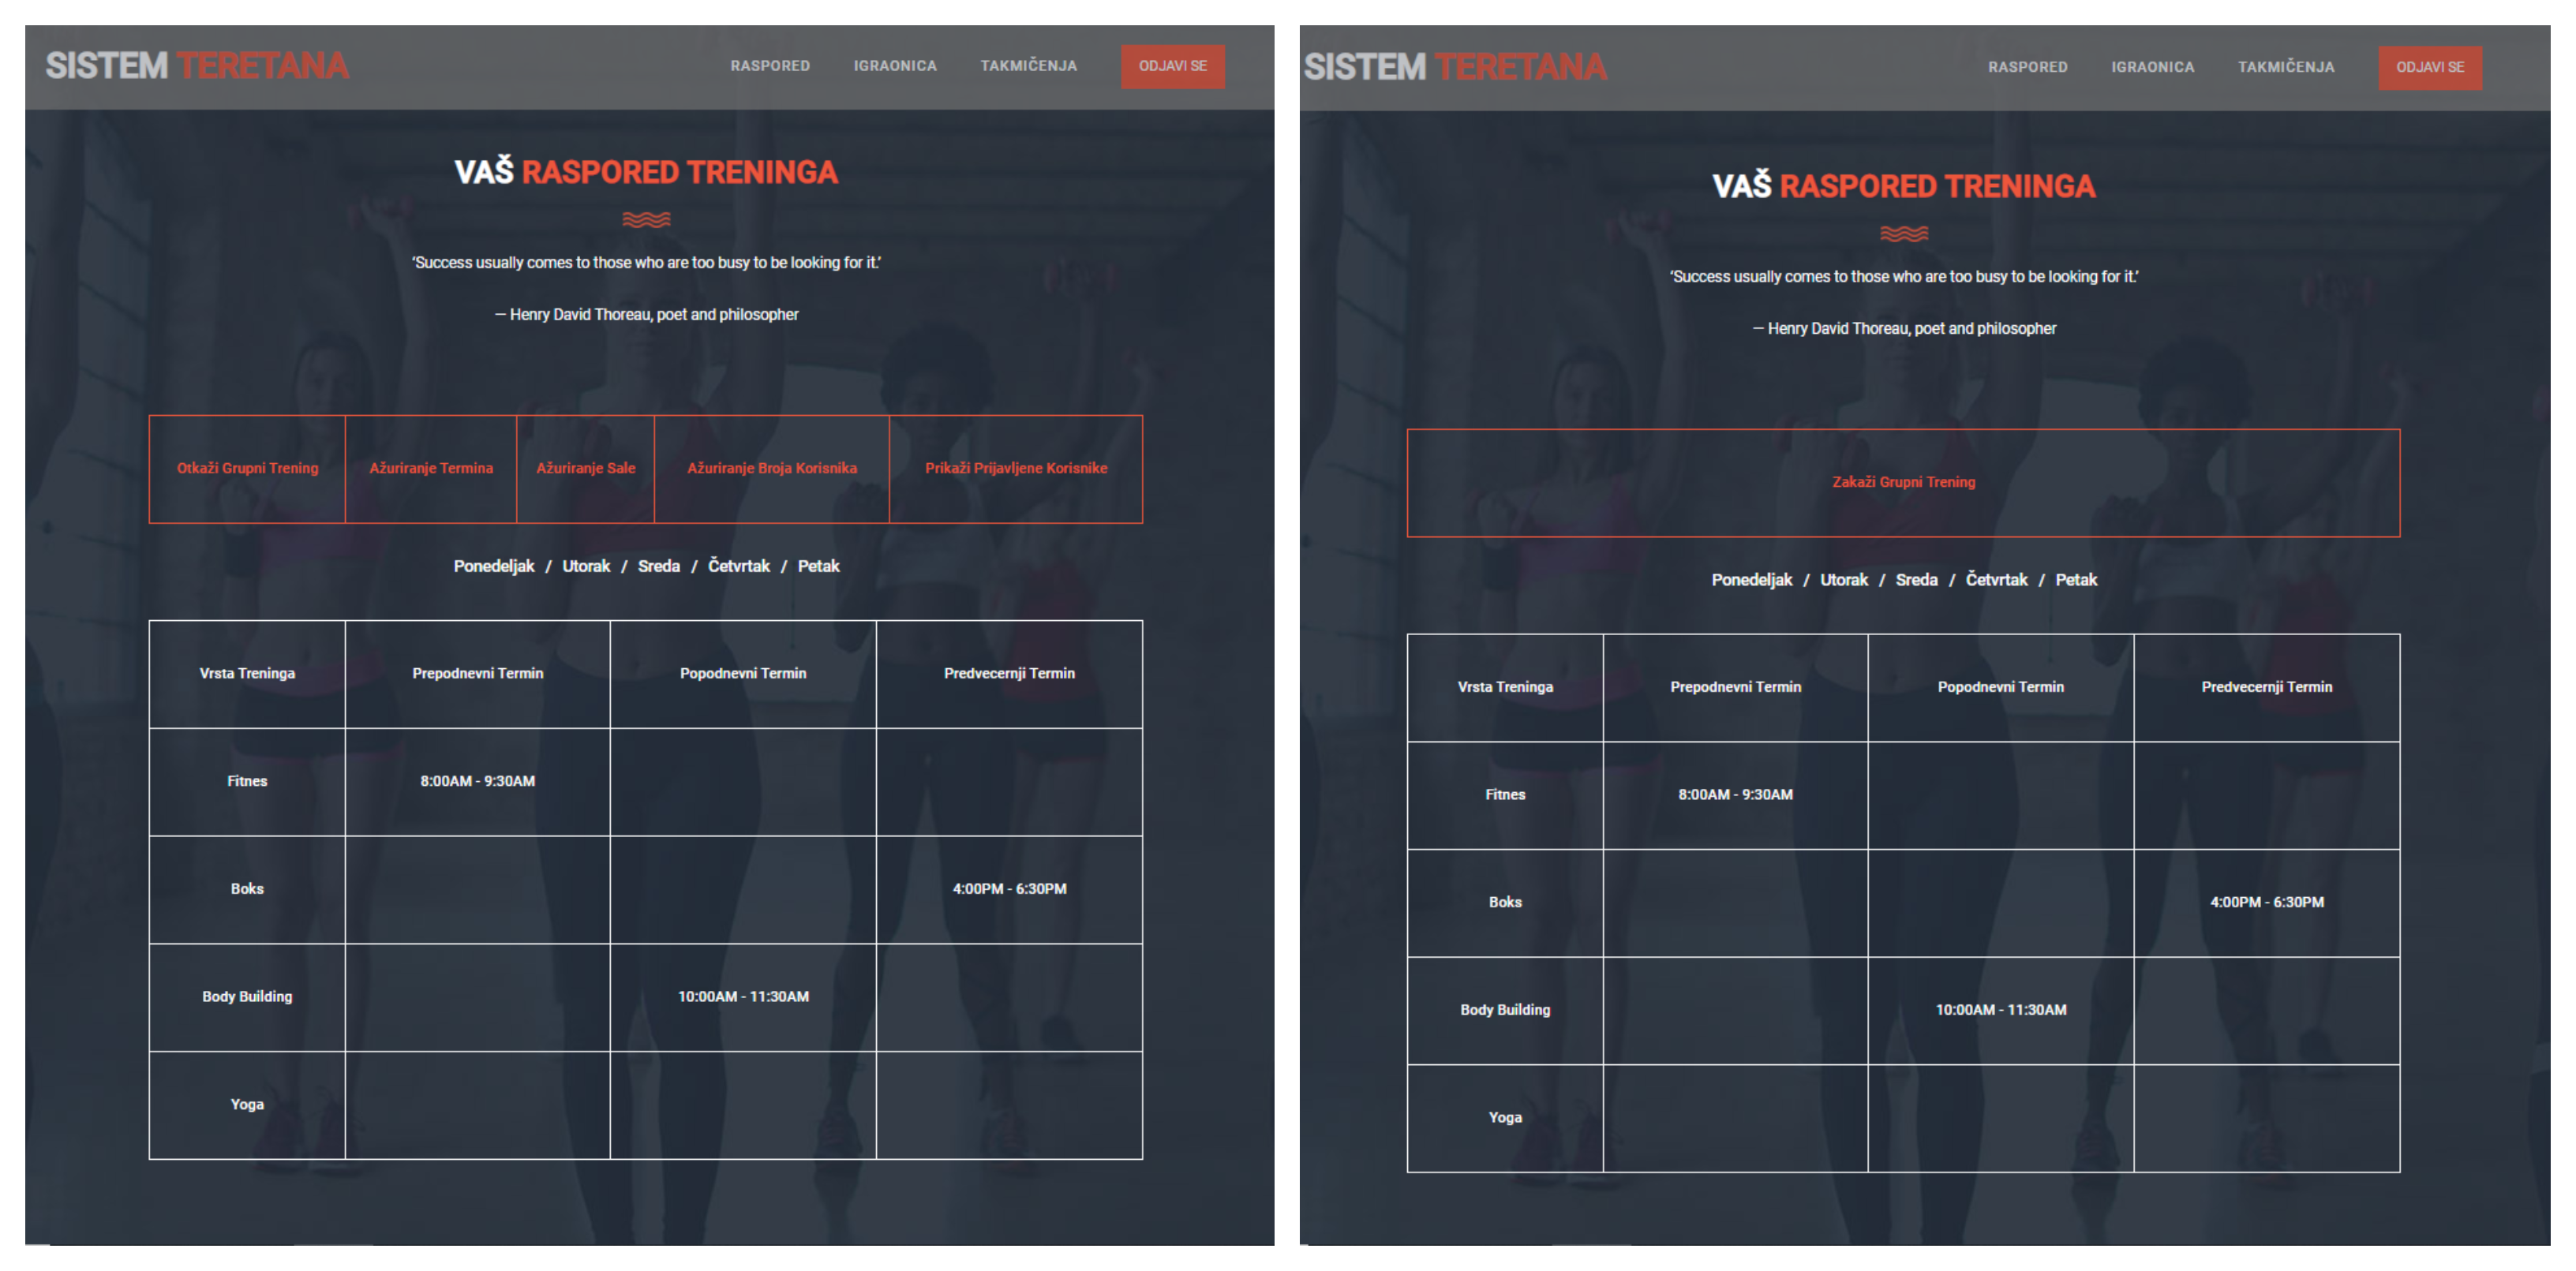
\includegraphics[scale=0.35]{sections/korisnicki_interfejs/screenshots/trener_raspored_toolbar.png}
\end{center}
\caption{ Traka sa alatkama: levo za kliknut zakazan termin, desno za nezakazan termin }
\label{fig:trener_toolbar}
\end{figure}

Klikom na svaku osim na ``Otkaži Grupni trening'' i ``Prikaži Prijavljene korisnike'' , otvara se odgovarajuća forma za menjanje informacija vezanim za dati trening(\ref{fig:trener_forme} prva, druga i treća). 
Klikom na ``Otkaži Grupni trening'' selektovani trening se briše i taj termin se oslobađa. 
Biranjem opcije ``Prikaži Prijavljene korisnike''(\ref{fig:trener_forme} četvrta) prikazuju se svi korisnici koji su prijavljeni na trening i dugme ``Preuzmi pdf''. Klikom dalje na to dugme skida se pdf u odgovarajućem formatu sa spiskom svih korisnika i njihovim informacijama, kako bi trener na narednom treningu mogao da vrši njihovu evaluaciju.

\begin{figure}[!ht]
\begin{center}
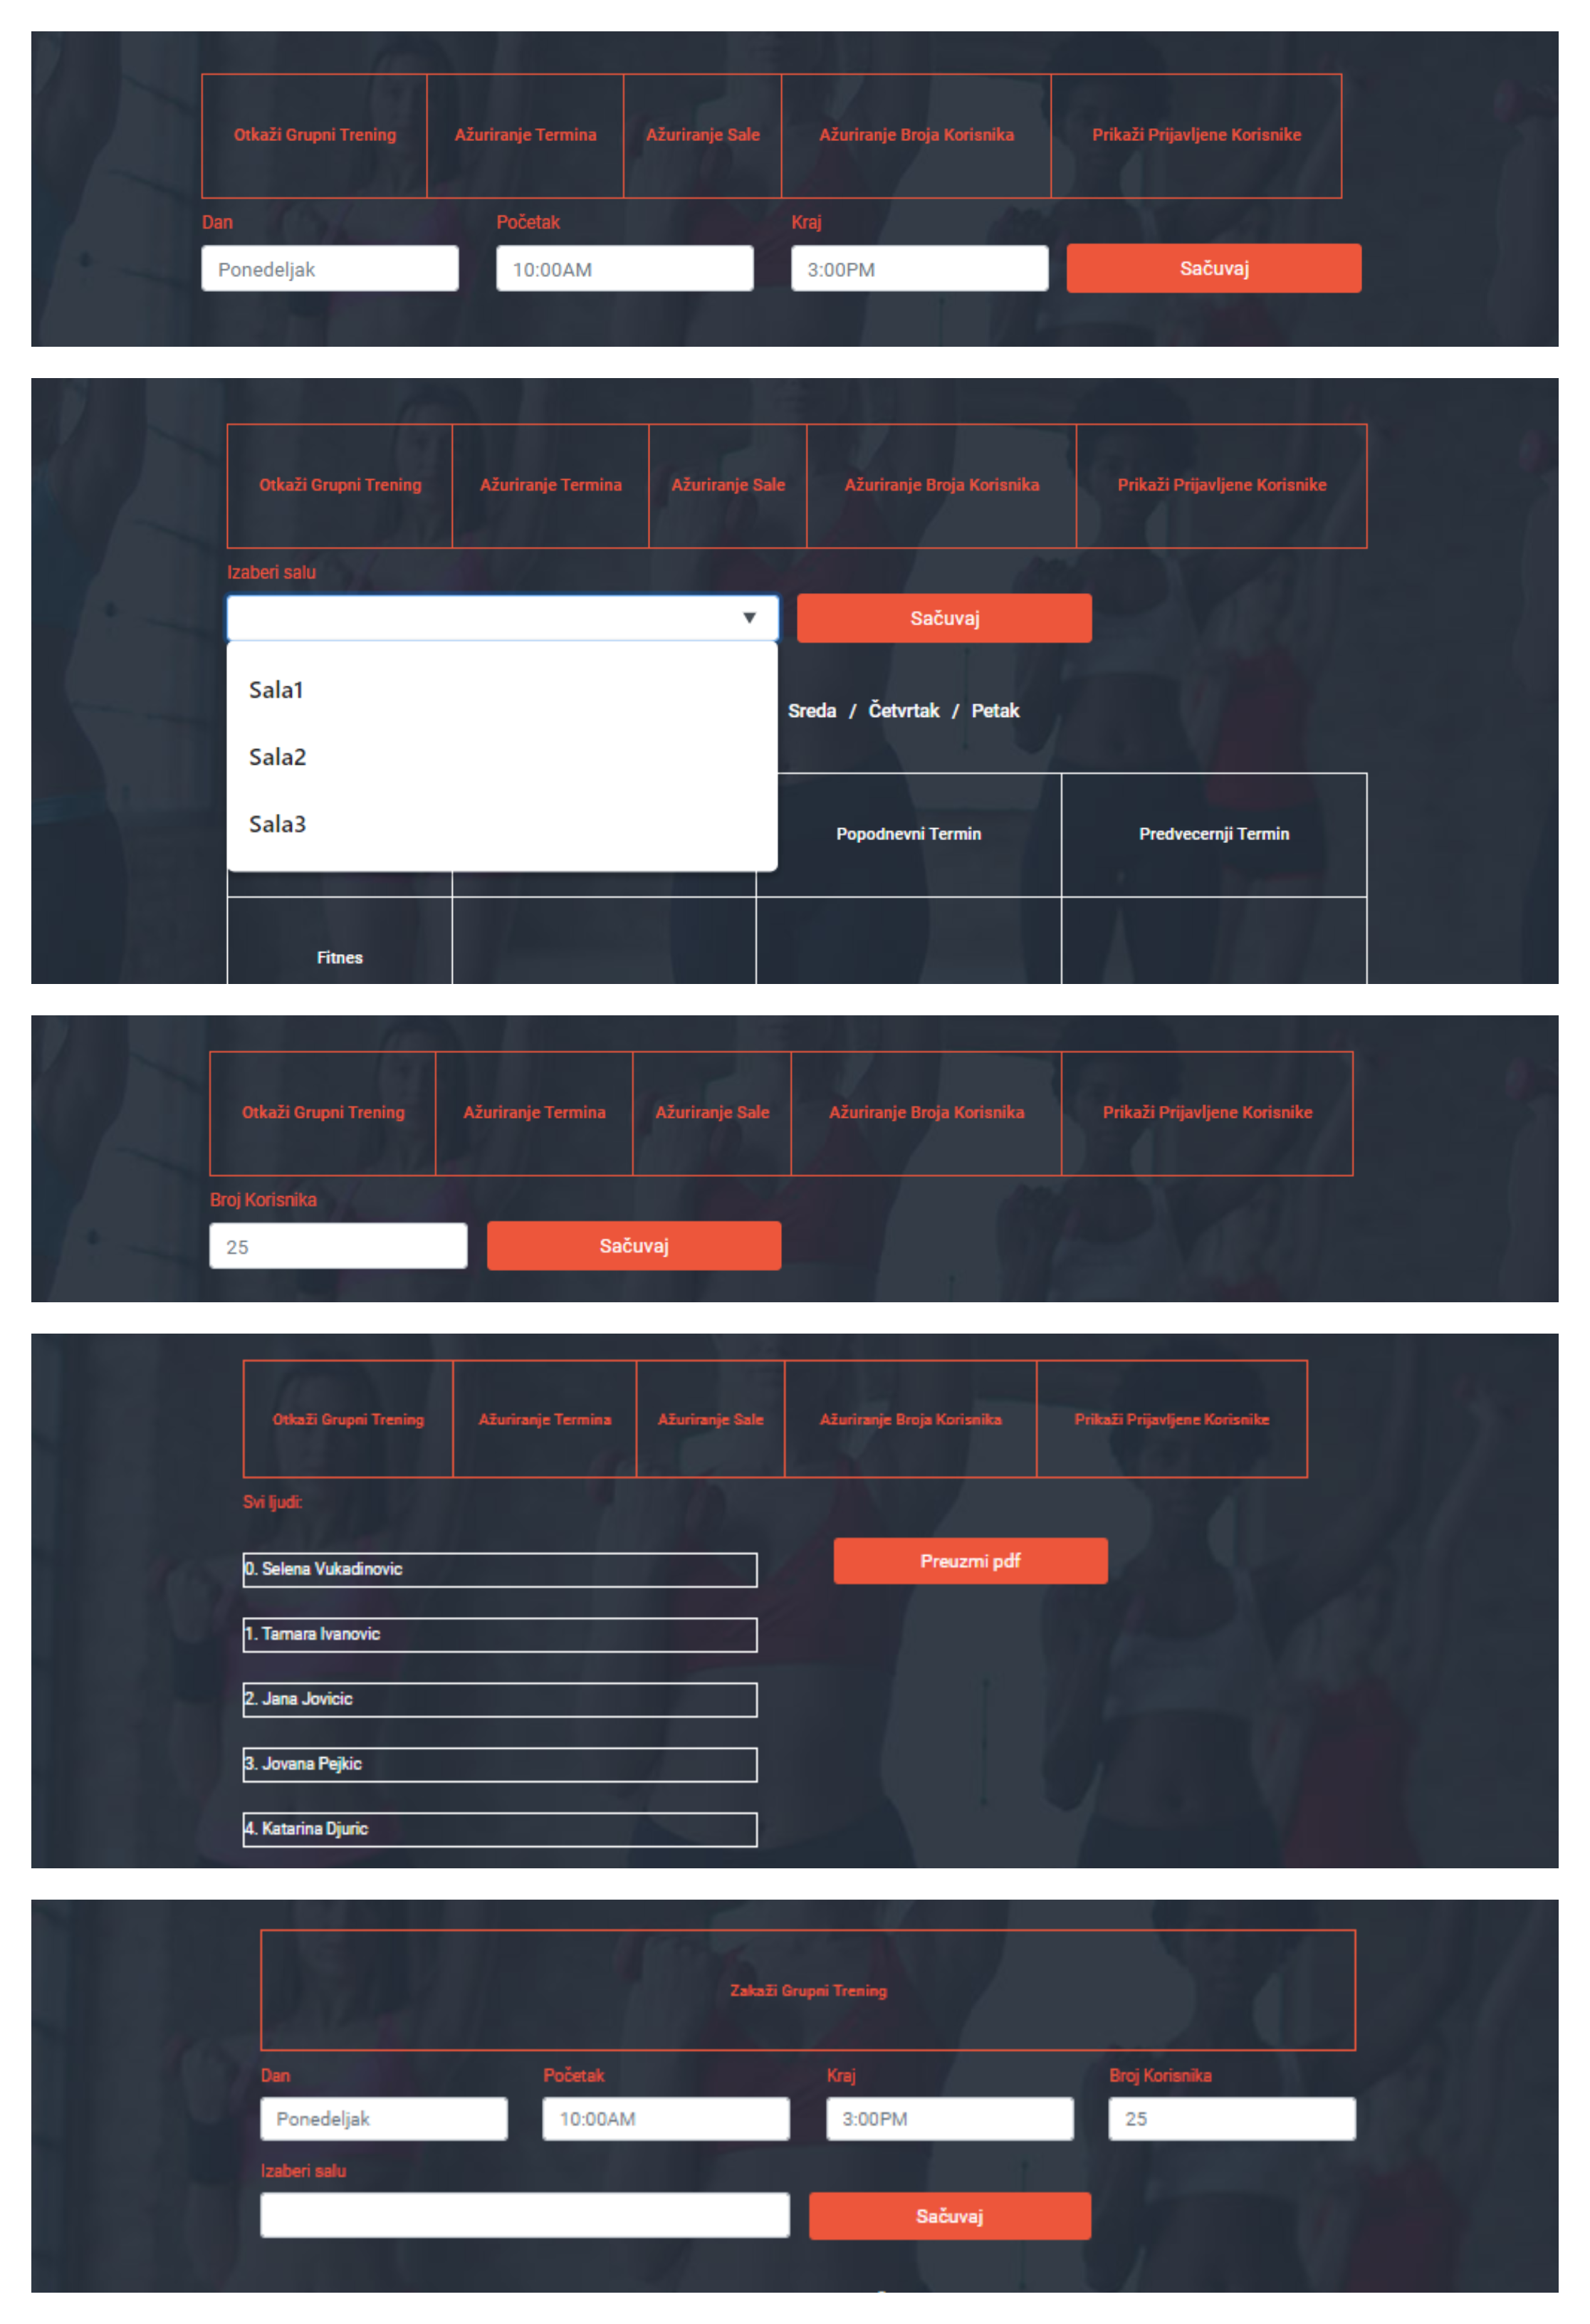
\includegraphics[scale=0.35]{sections/korisnicki_interfejs/screenshots/trener_raspored.png}
\end{center}
\caption{ Odozgo na dole: Forme za ažuriranje termina, ažuriranje sale, ažuriranje broja korisnika, pregled prijavljenih korisnika, forma za zakazivanje novog grupnog treninga }
\label{fig:trener_forme}
\end{figure}

\subsubsection{Raspored korisnika}
Klijent svoj raspored treninga vidi kao tabelu(\ref{fig:trener_forme} levo), sa opcijom da zakaže postojeći trening. Svako popunjeno polje u tabeli predstavlja postojeći trening na koji se korisnik prijavio, odnosno slobodan termin ukoliko se nije prijavio ni na jedan termin za dati vremenski period i datu vrstu treninga. Korisnik u jednom trenutku vidi svoj raspored treninga za jedan dan u nedelji(Inicijalno vidi za ponedeljak). Birajući dan u nedelji iznad tabele, može videti svoj raspored za taj dan.
Kada odabere dugme ``Zakaži trening'', iskače mu padajuća lista sa spiskom ponuđenih zakazanih treninga sortiranih po danu, pa po tipu treninga i na kraju po satu početka treninga(\ref{fig:trener_forme} desno).

\begin{figure}[!ht]
\begin{center}
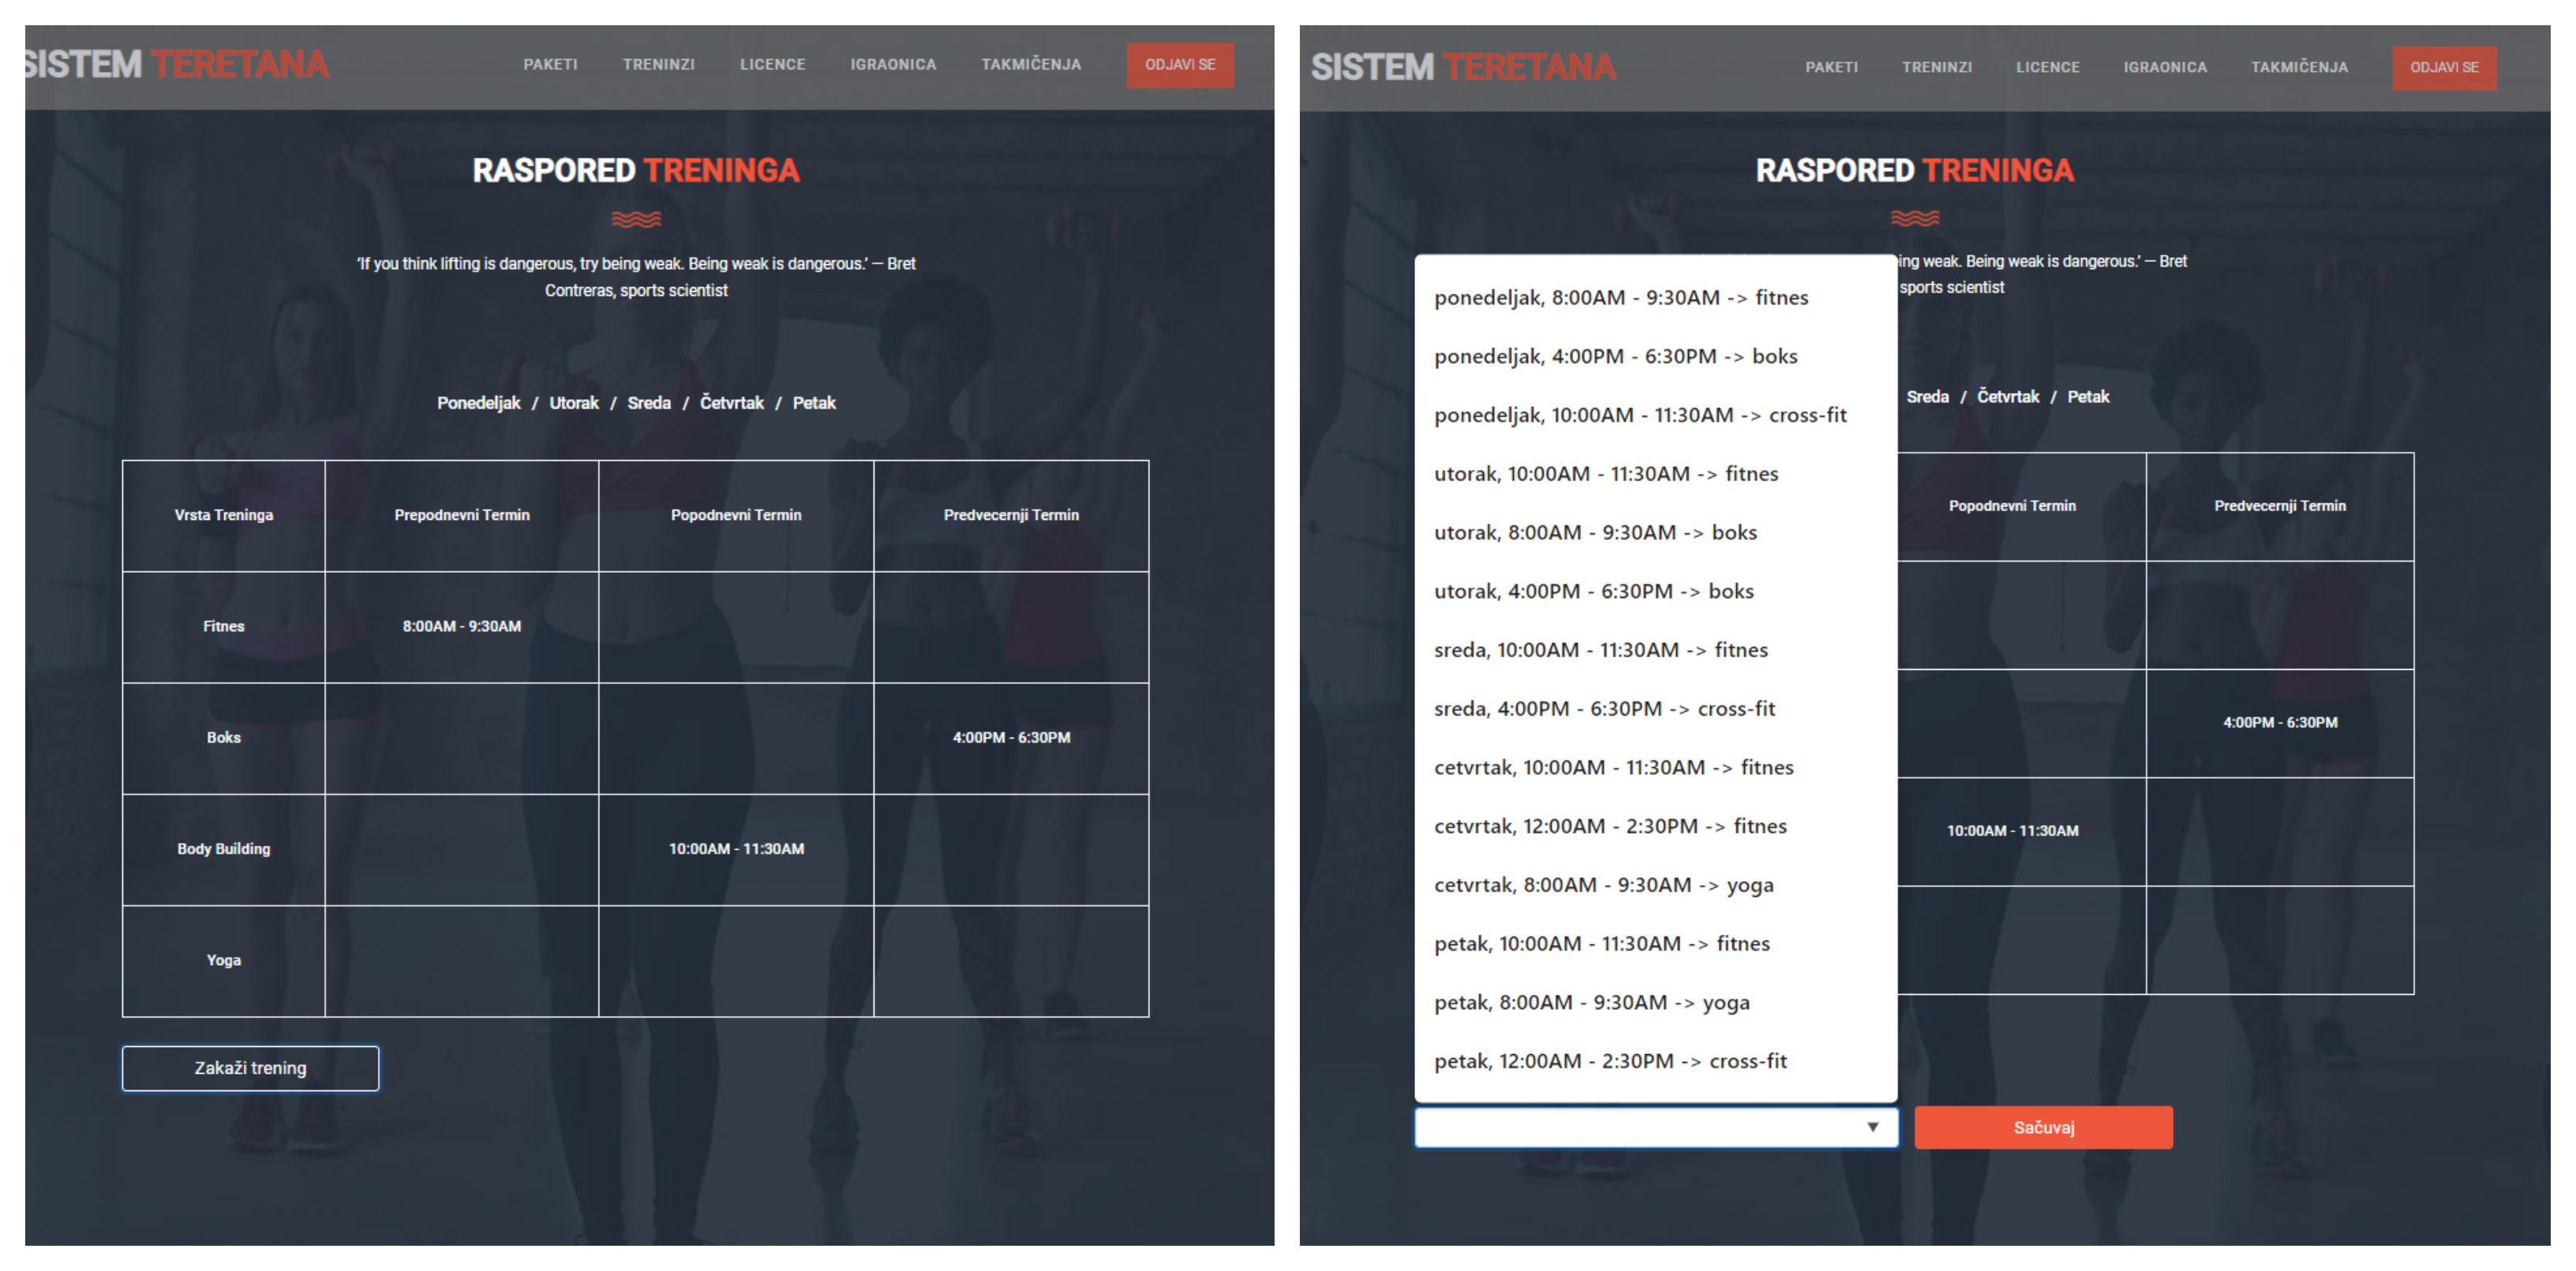
\includegraphics[scale=0.35]{sections/korisnicki_interfejs/screenshots/korisnik_raspored.png}
\end{center}
\caption{ Levo: raspored korisnika, Desno: prijavljivanje na trening }
\label{fig:trener_toolbar}
\end{figure}

\subsubsection{Treninzi i recepcioner}
Recepcioner ima uvid u sve zakazane treninge \ref{fig:recepcioner_pregled}. On, kao i ostali, zakazane treninge vidi kao tabelu i u jednom trenutku vidi zakazane treninge za jedan dan u nedelji(inicijalno ponedeljak).

\begin{figure}[!ht]
\begin{center}
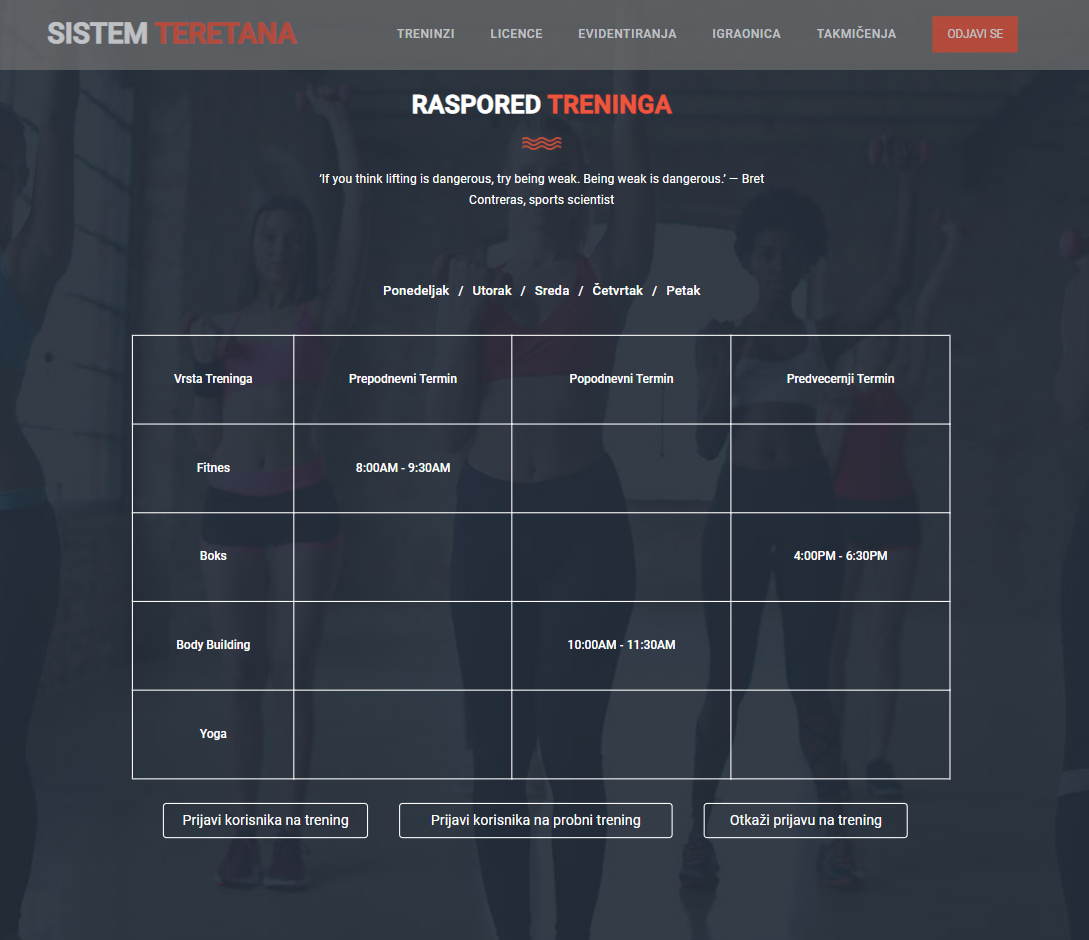
\includegraphics[scale=0.35]{sections/korisnicki_interfejs/screenshots/recepcioner_pregled_zakazanih_treninga.PNG}
\end{center}
\caption{Recepcioner pregled}
\label{fig:recepcioner_pregled}
\end{figure}

Biranjem opcije ``Prijavi korisnika na trening'' pojavljuju se dva radio dugmeta kojim se bira da li prijavljujemo korisnika na personalni ili gurpni trening. Zavisno od toga koja opcija je izabrana, prikazje se odgovarajuća forma \ref{fig:recepcioner_prijava} sa  padajućom listom termina i poljem za popunjavanje korisničkog imena. Polje za popunjenost nije moguće menjati i služi kao uvid u to koliko je još slobodnih mesta preostalo za zakazani trening.

\begin{figure}[!ht]
\begin{center}
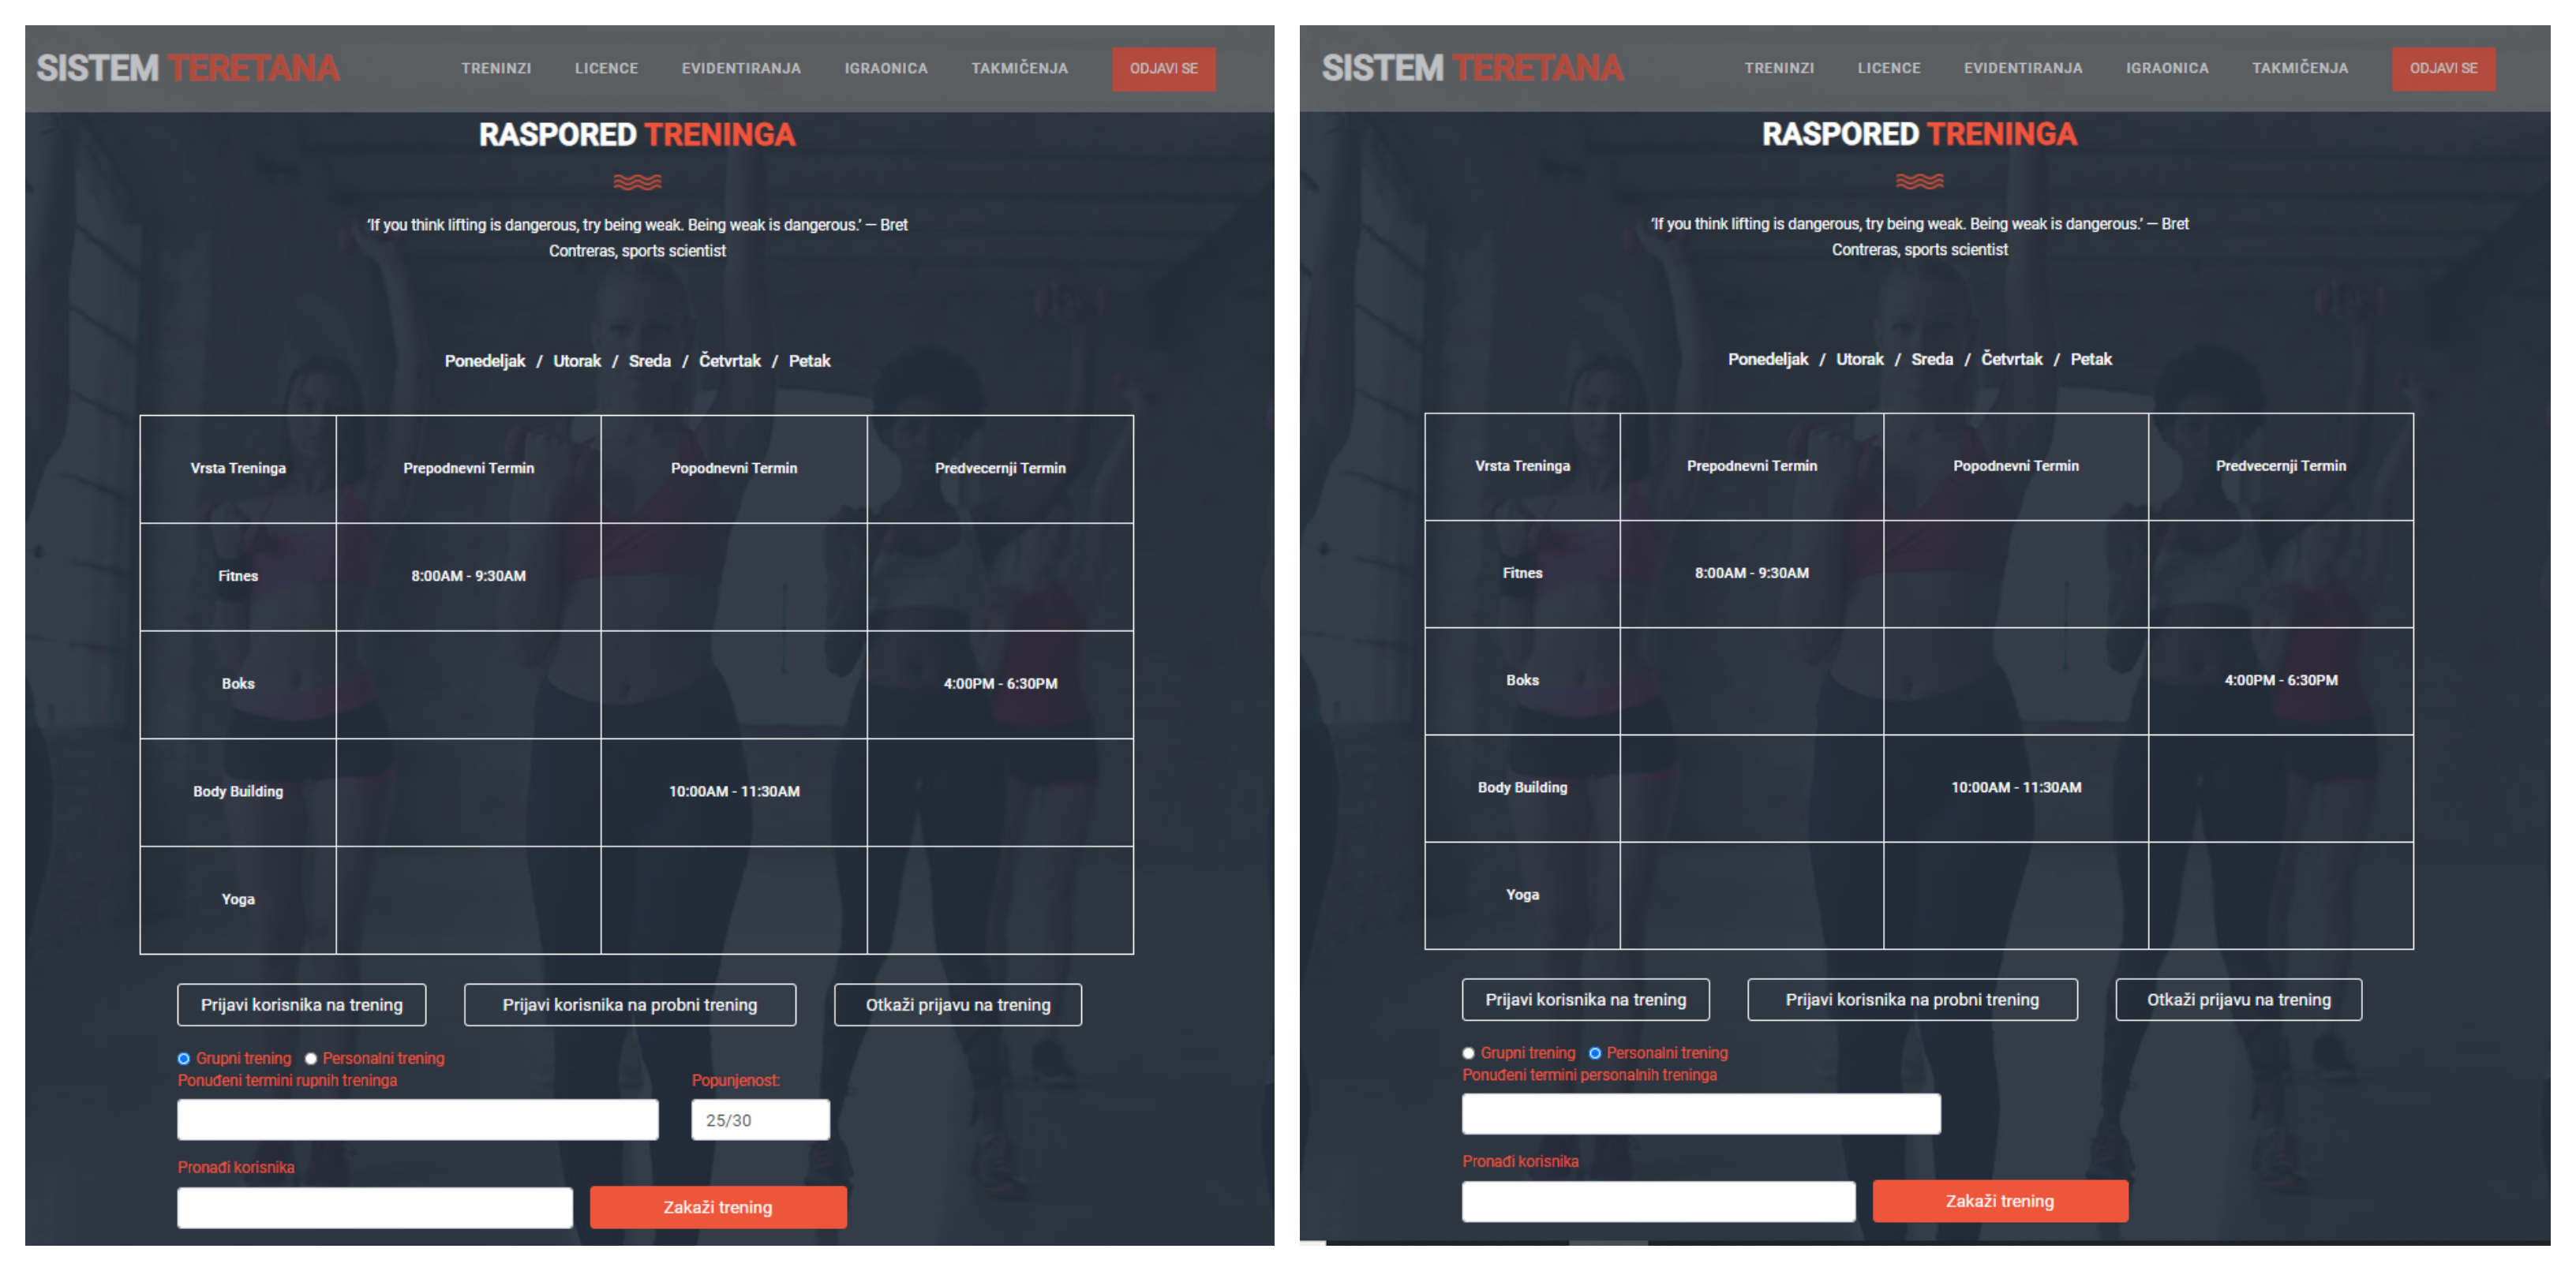
\includegraphics[scale=0.35]{sections/korisnicki_interfejs/screenshots/recepcioner_zakazi_trening.png}
\end{center}
\caption{ Levo: prijavljivanje na grupni trening, Desno: prijavljivanje na personalni trening }
\label{fig:recepcioner_prijava}
\end{figure}

Recepcioner može prijaviti korisnika i na probni trening klikom na dugme ``Prijavi korisnika na probni trening'' (\ref{fig:recepcioner_ostalo} levo). Svi probni treninzi su po pravilu grupni i prijavljeni korisnik se u evidenciji ne vodi kao da zauzima mesto, jer može da stoji sa strane i gleda. 
Za kraj, recepcioner na lični zahtev korisnika može da otkaže prijavu na trening biranjem opcije ``Otkaži prijavu na trening'' (\ref{fig:recepcioner_ostalo} levo), gde će recepcioner uneti odgovarajuće podatke o korisniku i treningu koji se otkazuje.

\begin{figure}[!ht]
\begin{center}
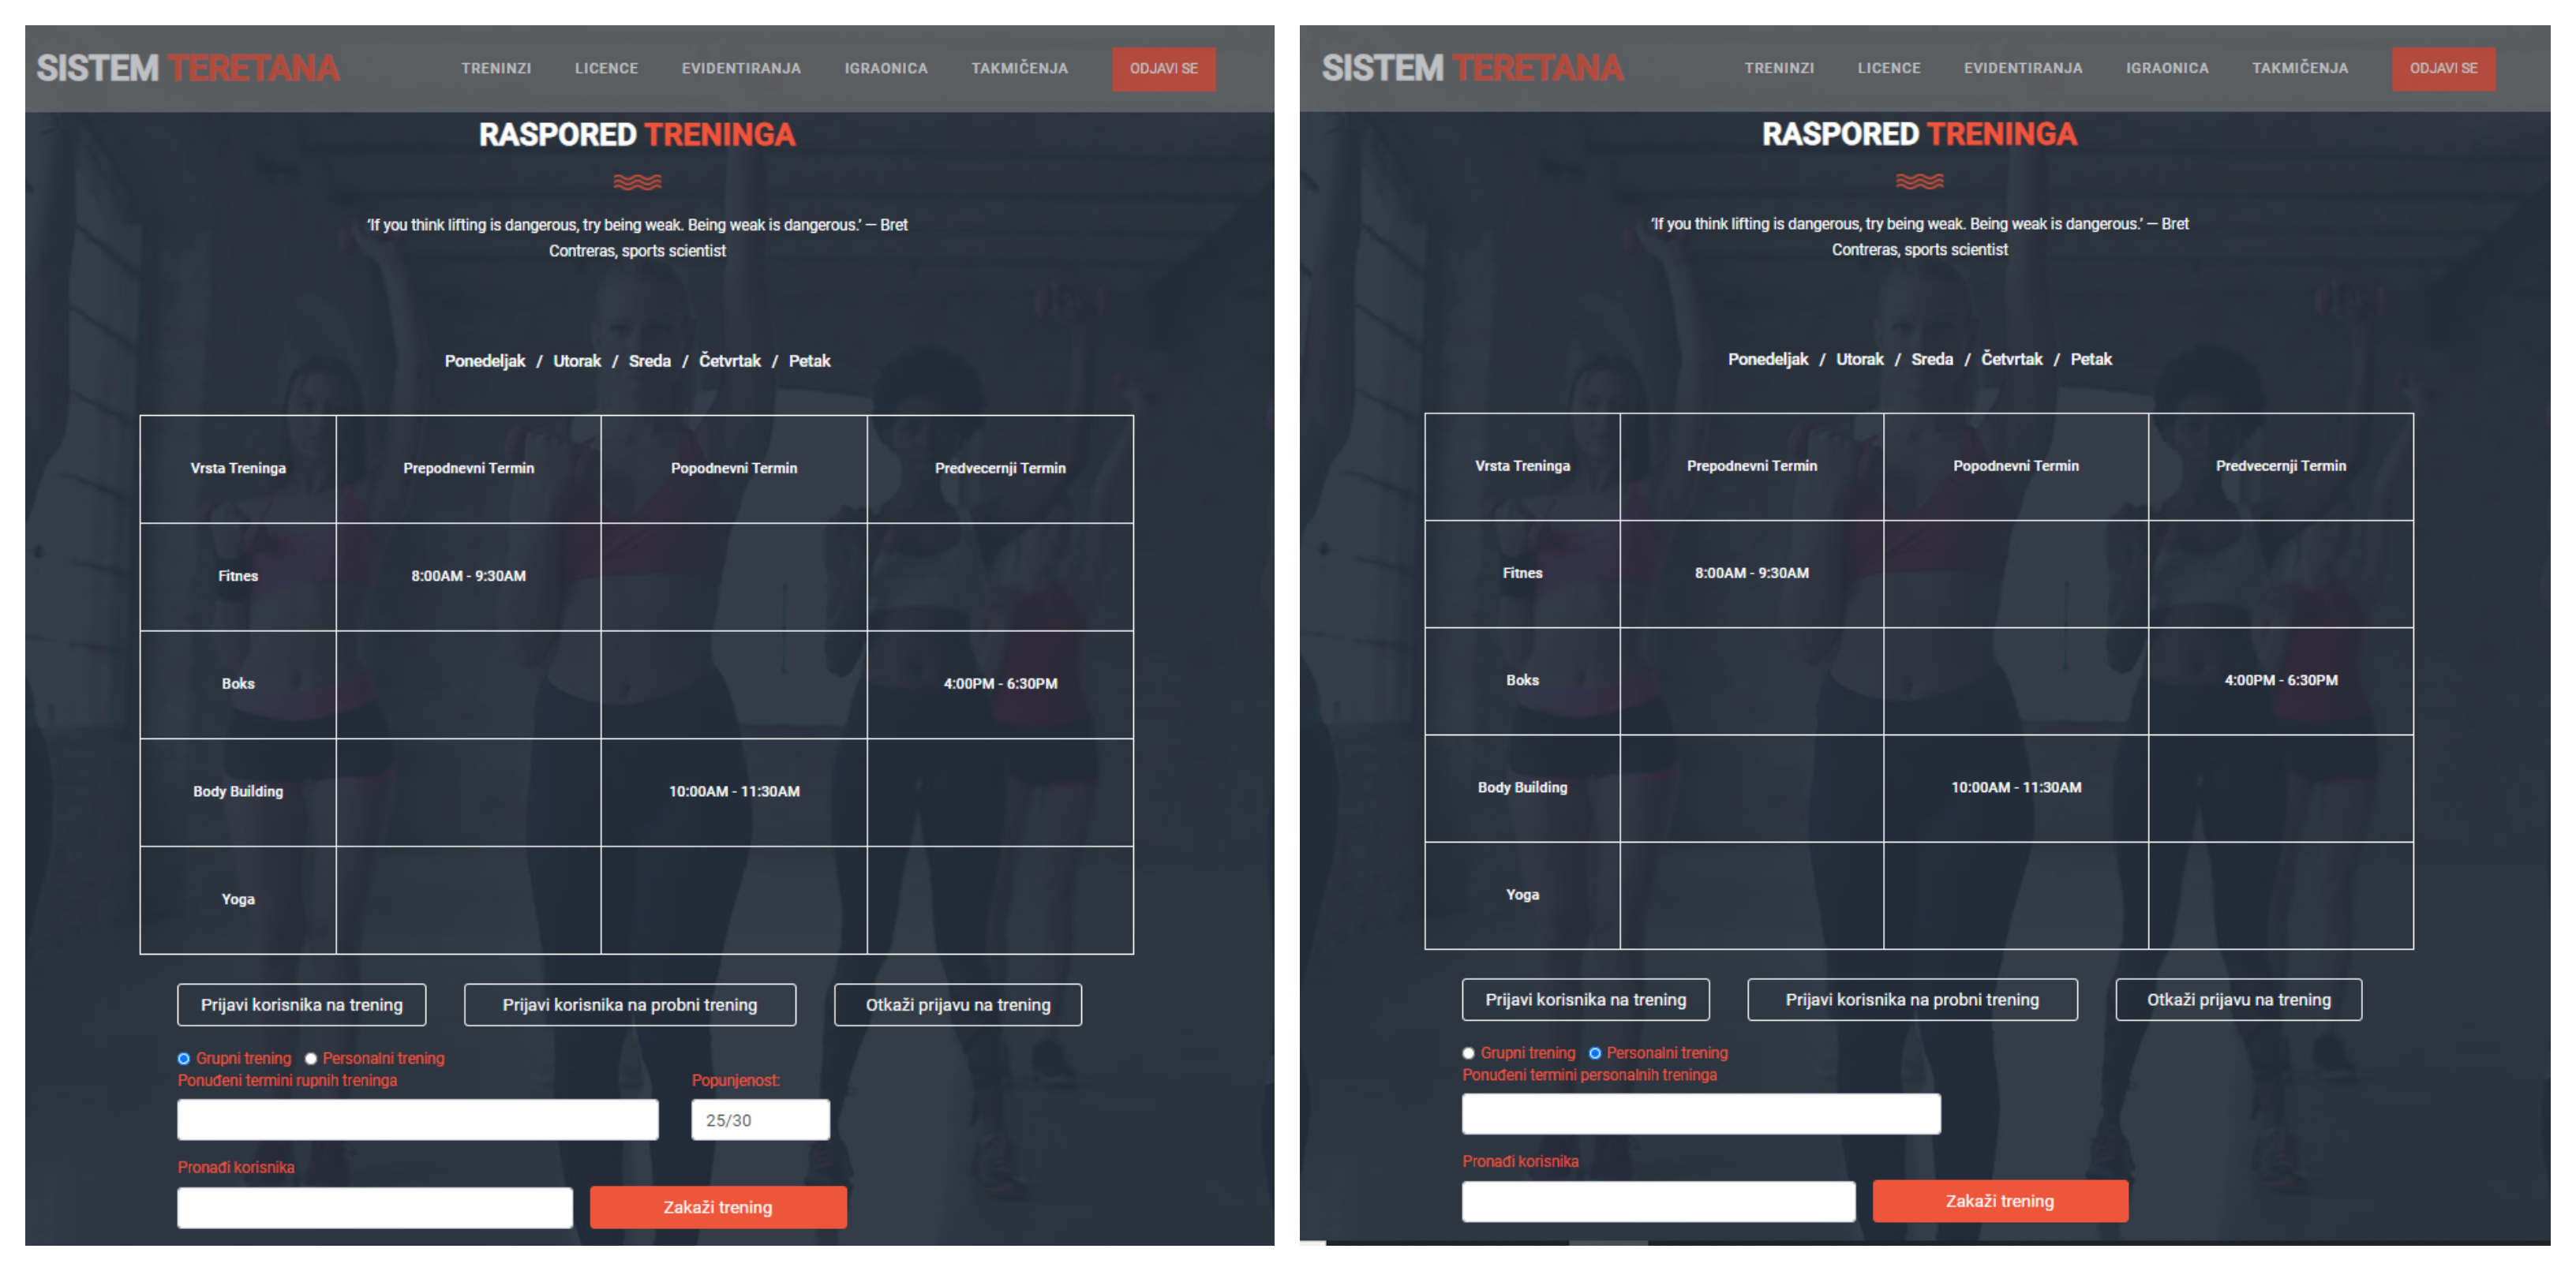
\includegraphics[scale=0.35]{sections/korisnicki_interfejs/screenshots/recepcioner_zakazi_trening.png}
\end{center}
\caption{ Levo: prijavljivanje na probni trening, Desno: otkazivanje prijave na trening }
\label{fig:recepcioner_ostalo}
\end{figure}


\end{document}